% !TEX program = xelatex
\documentclass[12pt,a4paper,twoside,openright]{book}

% ---- Page geometry (customization point: margins) ----
\usepackage[a4paper,inner=3.9cm,outer=3.5cm,top=3.2cm,bottom=3.4cm]{geometry}
\usepackage{setspace}
\setstretch{1.08}

% ---- Fonts: EB Garamond (text) + TeX Gyre Heros (headers, captions, section headings) ----
\usepackage{fontspec}
\defaultfontfeatures{Ligatures=TeX}
\setmainfont{EB Garamond}
\newfontfamily\lpHeadingFont{TeX Gyre Heros}

% ---- Packages ----
\usepackage{amsmath,amssymb}
\usepackage{graphicx}
\usepackage{booktabs}
\usepackage{multicol}
\usepackage{xcolor}
\usepackage{sectsty}
\usepackage{fancyhdr}
\usepackage[font=small,labelsep=period,justification=raggedright,singlelinecheck=false]{caption}
\usepackage{hyperref}

% ---- Palette (customization point: Design > Theme colors edits these) ----
\definecolor{lpAccent}{HTML}{7A2E3A}
\definecolor{lpBody}{HTML}{1E1B1A}
\definecolor{lpChapter}{HTML}{3F2A2E}
\definecolor{lpSection}{HTML}{5B3A3F}
\definecolor{lpSubsection}{HTML}{6B5B4E}
\definecolor{lpSubsubsection}{HTML}{6B5B4E}
\AtBeginDocument{\color{lpBody}}
\hypersetup{colorlinks=true,linkcolor=lpAccent,citecolor=lpAccent,urlcolor=lpAccent}
\hypersetup{linktoc=page,pdftitle={Title of the Book or Report},pdfauthor={Author Name}}

% ---- Book metadata (customization point: edit these, used by the front-matter pages) ----
\title{Title of the Book or Report}
\newcommand{\booksubtitle}{An Illustrative Subtitle for the Volume}
\author{Author Name}
\newcommand{\authoraffiliation}{Department of Studies, University Name}
\newcommand{\authoremail}{email@example.org}
\newcommand{\bookpublisher}{Publisher Name}
\newcommand{\bookplace}{City}
\newcommand{\bookisbn}{000-0-00-000000-0}
\date{}

% ---- Text rhythm ----
\setlength{\parindent}{1.4em}
\setlength{\parskip}{0pt plus 0.4pt}
\clubpenalty=10000
\widowpenalty=10000
\displaywidowpenalty=10000
\setcounter{secnumdepth}{2}
\setcounter{tocdepth}{1}
\numberwithin{equation}{chapter}

% ---- Headings: sans-serif section heads (Heros); chapter openings are set below ----
\sectionfont{\lpHeadingFont\color{lpSection}}
\subsectionfont{\lpHeadingFont\color{lpSubsection}}
\subsubsectionfont{\lpHeadingFont\color{lpSubsubsection}}
\chapterfont{\color{lpChapter}}

% ---- Running headers and footers (customization point) ----
\pagestyle{fancy}
\fancyhf{}
\fancyhead[LE,RO]{\lpHeadingFont\footnotesize\thepage}
\fancyhead[RE]{\lpHeadingFont\footnotesize\nouppercase{\leftmark}}
\fancyhead[LO]{\lpHeadingFont\footnotesize\nouppercase{\rightmark}}
\renewcommand{\headrulewidth}{0.3pt}
\setlength{\headheight}{14pt}

% ---- Captions ----
\DeclareCaptionFont{heros}{\lpHeadingFont}
\captionsetup{labelfont={heros,bf}}

\makeatletter
% Heading sizes (class defaults are too large for Garamond at 12 pt)
\renewcommand\Large{\@setfontsize\Large{15}{19}}
\renewcommand\large{\@setfontsize\large{13}{16}}

% Running-head marks: "Title" on verso pages, "1.2 Section" on recto pages
\renewcommand{\chaptermark}[1]{\markboth{#1}{}}
\renewcommand{\sectionmark}[1]{\markright{\thesection\quad #1}}

% Blank pages inserted before a recto page carry no header or footer
\renewcommand{\cleardoublepage}{\clearpage\if@twoside\ifodd\c@page\else\hbox{}\thispagestyle{empty}\newpage\fi\fi}

% Letter-spaced text for labels and title pages
\newcommand{\lpSpaced}[1]{{\addfontfeature{LetterSpace=14}#1}}

% Chapter openings (customization point): label, large title, short accent rule
\renewcommand{\@makechapterhead}[1]{%
  \vspace*{3\baselineskip}%
  {\raggedright\normalfont
   \ifnum\c@secnumdepth>\m@ne
     {\color{lpAccent}\lpHeadingFont\footnotesize\lpSpaced{\MakeUppercase{\@chapapp}\ \thechapter}\par}%
     \vskip 9\p@
   \fi
   {\color{lpChapter}\fontsize{27}{31}\selectfont #1\par}%
   \vskip 7\p@
   {\color{lpAccent}\hrule width 2.5cm height 0.6pt}%
   \nobreak\vskip 3\baselineskip}}
\renewcommand{\@makeschapterhead}[1]{%
  \vspace*{3\baselineskip}%
  {\raggedright\normalfont
   {\color{lpChapter}\fontsize{27}{31}\selectfont #1\par}%
   \vskip 7\p@
   {\color{lpAccent}\hrule width 2.5cm height 0.6pt}%
   \nobreak\vskip 3\baselineskip}}

% Front-matter pages: call these in the body, in this order (customization point)
\newcommand{\halftitlepage}{%
  \cleardoublepage\thispagestyle{empty}%
  \null\vfill
  {\centering\color{lpChapter}\fontsize{24}{29}\selectfont\@title\par}%
  \vfill\vfill\clearpage}
\newcommand{\fulltitlepage}{%
  \cleardoublepage\thispagestyle{empty}%
  \vspace*{0.12\textheight}%
  {\centering
   {\color{lpAccent}\rule{2.2cm}{0.6pt}\par}\vspace{1.6cm}%
   {\color{lpChapter}\fontsize{34}{40}\selectfont\@title\par}\vspace{0.6cm}%
   {\color{lpSection}\itshape\fontsize{16}{20}\selectfont\booksubtitle\par}\vspace{1.6cm}%
   {\color{lpAccent}\rule{2.2cm}{0.6pt}\par}\vspace{1.4cm}%
   {\scshape\fontsize{16}{20}\selectfont\lpSpaced{\@author}\par}\vspace{0.3cm}%
   {\small\itshape\authoraffiliation\par}}%
  \vfill
  {\centering\lpHeadingFont\scriptsize\lpSpaced{\MakeUppercase{\bookpublisher}}\par\vspace{3pt}%
   \bookplace\ \textperiodcentered\ \the\year\par}%
  \clearpage}
\newcommand{\copyrightpage}{%
  \clearpage\thispagestyle{empty}\vspace*{\fill}%
  {\footnotesize\setlength{\parindent}{0pt}\setlength{\parskip}{0.6em}\raggedright
   Copyright \copyright\ \the\year\ \@author. All rights reserved.\par
   First edition, \the\year. Published by \bookpublisher, \bookplace.\par
   ISBN \bookisbn\par
   Author contact: \authoremail\par
   Typeset with XeLaTeX in EB Garamond and TeX Gyre Heros.\par}%
  \clearpage}
\newcommand{\bookdedication}[1]{%
  \cleardoublepage\thispagestyle{empty}%
  \null\vfill
  {\centering\itshape\large #1\par}%
  \vfill\vfill\clearpage}

% Epigraph at the start of a chapter: \chapterepigraph{Quoted text}{Source}
\newcommand{\chapterepigraph}[2]{%
  \begin{flushright}\begin{minipage}{0.72\textwidth}\raggedleft\small\itshape #1\par
  \vspace{3pt}\upshape\scshape #2\par\end{minipage}\end{flushright}\vspace{1.5\baselineskip}}

% Block quotations
\renewenvironment{quote}
  {\list{}{\listparindent\z@\itemindent\z@\leftmargin2.2em\rightmargin2.2em\topsep0.8\baselineskip\parsep\z@\@plus\p@}\item\relax\small}
  {\endlist}
\makeatother

\begin{document}

% ================= FRONT MATTER =================
\frontmatter
\halftitlepage
\fulltitlepage
\copyrightpage
\bookdedication{For those who read the footnotes.}

\chapter*{Preface}
This volume grew out of a simple question: how do we describe change across a body of
writing without losing sight of its individual works? The preface is the place to state
the book's origin, its intended readers, and the debts incurred along the way.

Replace this text with your own. Add acknowledgments, notes on editions and translations,
and any conventions the reader should know before beginning.

\tableofcontents
\listoffigures
\listoftables

\chapter{List of Abbreviations}\label{chap:abbr}
{\renewcommand{\arraystretch}{1.3}\small
\begin{tabular}{@{}p{0.2\textwidth}p{0.68\textwidth}@{}}
  DOI  & Digital Object Identifier \\
  ISBN & International Standard Book Number \\
  MS   & Manuscript \\
  ed.  & Editor, edited by \\
  cf.  & Compare (\emph{confer}) \\
\end{tabular}}

% ================= MAIN MATTER =================
\mainmatter

\chapter{Introduction}\label{chap:intro}
\chapterepigraph{A book must be an ice-axe to break the sea frozen inside us.}{Franz Kafka}

\section{Background}\label{sec:background}
Open the book by situating the subject within existing scholarship~\cite{smith2001}.
A well-formed introduction states the problem, the argument, and the structure of what
follows.\footnote{Footnotes are set in the smaller size below the text block and are
numbered continuously within each chapter.}

Scholars have long argued over how best to read such material. One influential statement
of the problem runs as follows:
\begin{quote}
  Block quotations are set smaller and indented on both sides, without quotation marks.
  Use them for passages longer than about three lines.
  \par\raggedleft\upshape\scshape Author, \emph{Title} (2001), p.~12
\end{quote}
The argument developed here responds to that position.

\section{Scope and Method}\label{sec:scope}
Chapter~\ref{chap:framework} introduces the conceptual framework, and
Chapter~\ref{chap:analysis} applies it to the corpus described below.

\subsection{Corpus}\label{sec:corpus}
Describe the sources, selection criteria and any limits of the evidence. The illustrative
corpus used throughout this template contains one thousand works
(Table~\ref{tab:summary}).

\subsection{Analytical approach}
Outline the procedure in enough detail that another scholar could repeat it~\cite{jones2010}.
Add further sections and subsections with \verb|\section| and \verb|\subsection|.

\chapter{Theoretical Framework}\label{chap:framework}

\section{Core Concepts}
Define the key terms once, then use them consistently. Concepts introduced here are
applied in Chapter~\ref{chap:analysis}.

\section{A Simple Growth Model}\label{sec:growth}
Cumulative output often follows a saturating pattern. Let $N(t)$ be the number of works
at time $t$, $r$ a growth rate and $K$ the carrying capacity:
\begin{equation}\label{eq:growth}
  \frac{\mathrm{d}N}{\mathrm{d}t} = r\,N\!\left(1-\frac{N}{K}\right),
  \qquad
  N(t) = \frac{K}{1+e^{-r(t-t_0)}}.
\end{equation}
Equation~\eqref{eq:growth} is derived in Appendix~\ref{app:derivation}, and
Figure~\ref{fig:growth} shows an illustrative curve.

\begin{figure}[htbp]
  \centering
  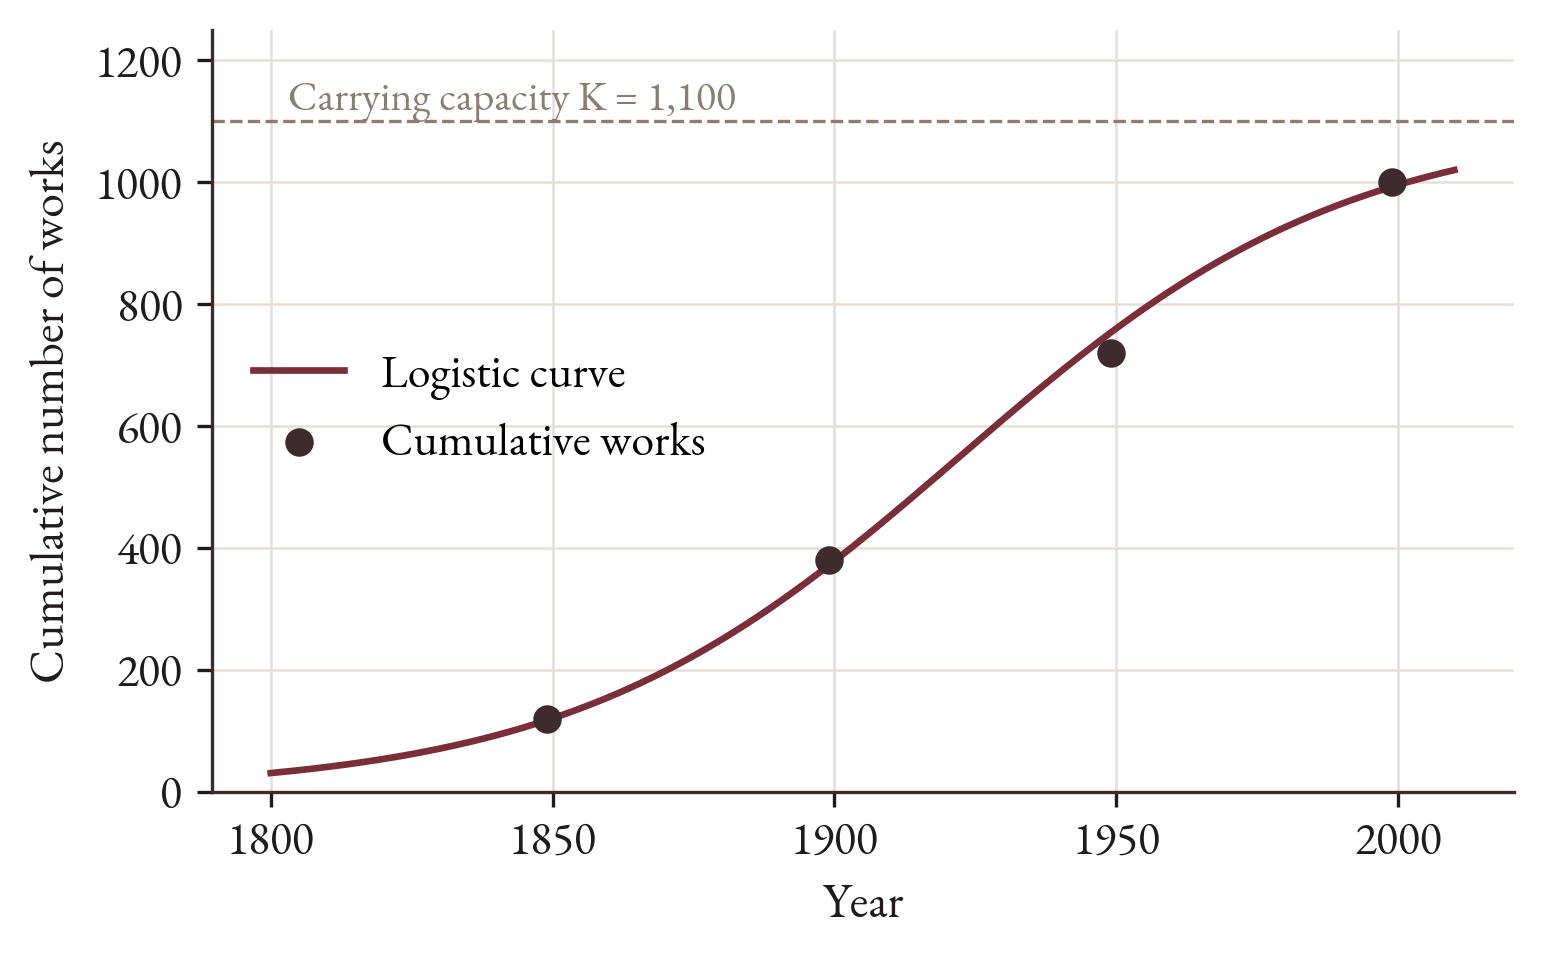
\includegraphics[width=0.85\textwidth]{figures/book-growth.png}
  \caption{Cumulative works by period (illustrative data) with a logistic curve fitted on
  the logit scale, carrying capacity fixed at 1,100.}\label{fig:growth}
\end{figure}

\chapter{Analysis}\label{chap:analysis}

\section{Descriptive Results}
Table~\ref{tab:summary} summarises the corpus by period; the values are placeholders to
be replaced with your own data.

\begin{table}[htbp]
  \centering
  \caption{Illustrative corpus by period (placeholder values).}\label{tab:summary}
  \small
  \begin{tabular}{@{}lrrr@{}}
    \toprule
    Period & Works & Mean length (pages) & Share (\%) \\
    \midrule
    1800--1849 & 120 & 310 & 12.0 \\
    1850--1899 & 260 & 335 & 26.0 \\
    1900--1949 & 340 & 352 & 34.0 \\
    1950--1999 & 280 & 371 & 28.0 \\
    \midrule
    Total & 1\,000 & 348 & 100.0 \\
    \bottomrule
  \end{tabular}
\end{table}

\section{Distribution by Category}\label{sec:category}
Figure~\ref{fig:categories} shows how the works divide by category; the underlying counts
are listed in Table~\ref{tab:categories} (Appendix~\ref{app:data}).

\begin{figure}[htbp]
  \centering
  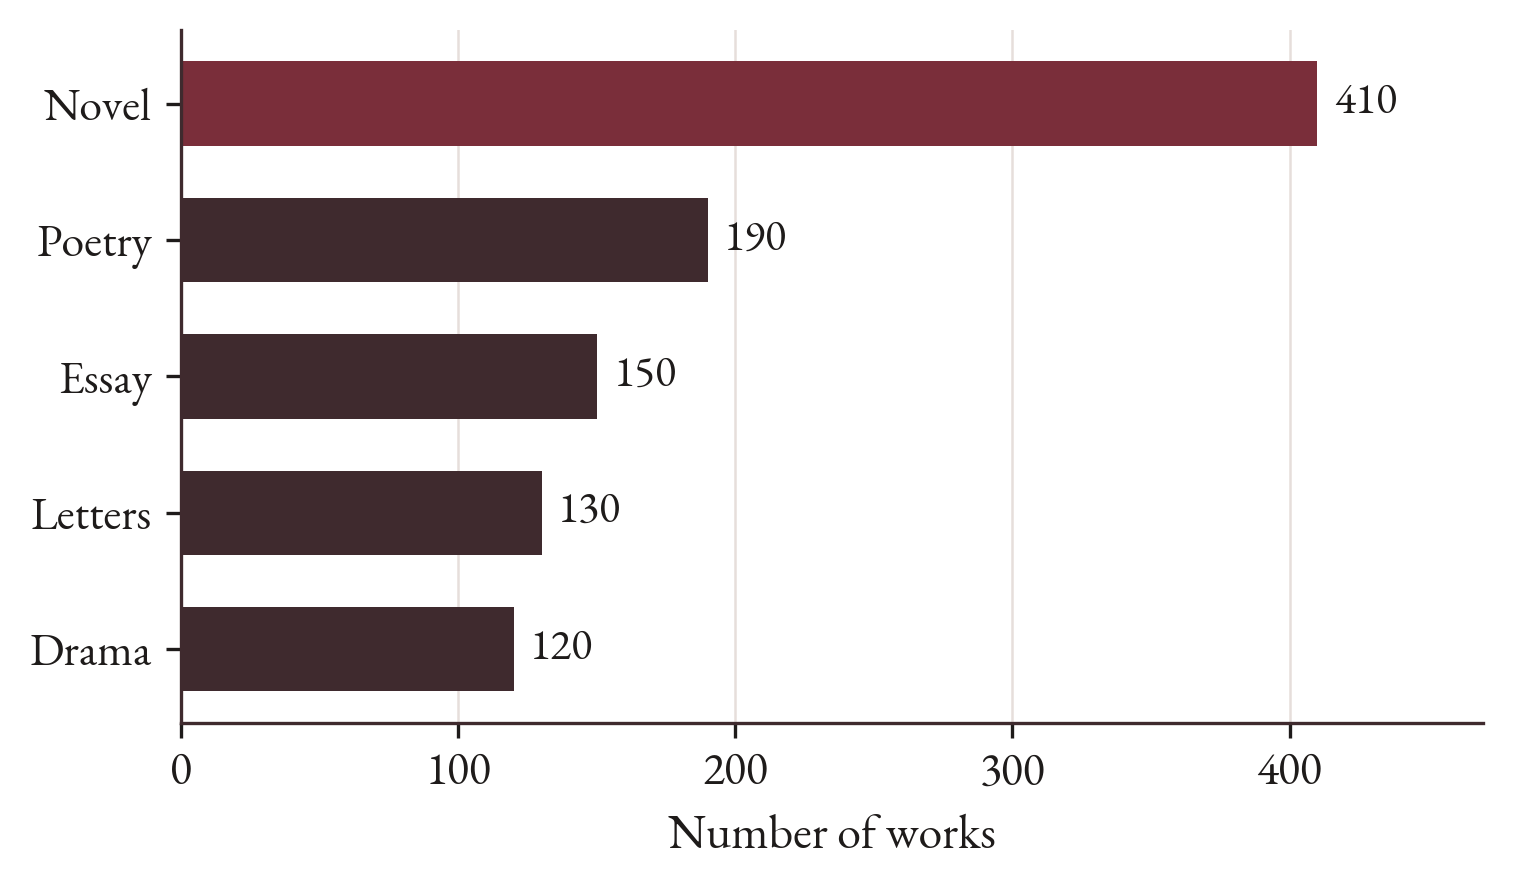
\includegraphics[width=0.85\textwidth]{figures/book-categories.png}
  \caption{Works by category (illustrative data).}\label{fig:categories}
\end{figure}

\section{Interpretation}
Discuss what the results mean for the argument~\cite{lee2018}, noting limitations and
alternative readings.

% ================= BACK MATTER =================
\chapter*{Conclusion}
\markboth{Conclusion}{}
\phantomsection\addcontentsline{toc}{chapter}{Conclusion}
Summarise the argument and its contribution, return to the questions posed in
Chapter~\ref{chap:intro}, and indicate directions for future work.

\appendix
\chapter{Derivation of the Growth Model}\label{app:derivation}
Starting from the logistic equation in Equation~\eqref{eq:growth}, separate variables:
\begin{align}
  \frac{\mathrm{d}N}{N\,(1-N/K)} &= r\,\mathrm{d}t, \\
  \ln\frac{N}{K-N} &= r\,(t-t_0).
\end{align}
Solving for $N$ yields the closed form quoted in the main text.

\chapter{Supplementary Data}\label{app:data}
\begin{table}[htbp]
  \centering
  \caption{Works by category (illustrative values).}\label{tab:categories}
  \small
  \begin{tabular}{@{}lrr@{}}
    \toprule
    Category & Works & Share (\%) \\
    \midrule
    Novel   & 410 & 41.0 \\
    Poetry  & 190 & 19.0 \\
    Essay   & 150 & 15.0 \\
    Letters & 130 & 13.0 \\
    Drama   & 120 & 12.0 \\
    \bottomrule
  \end{tabular}
\end{table}

\backmatter

\begin{thebibliography}{99}
\addcontentsline{toc}{chapter}{\bibname}
\bibitem{smith2001} A.~Smith, \emph{Title of a Foundational Study} (City: Publisher, 2001).
\bibitem{jones2010} B.~Jones, ``Title of an Article,'' \emph{Journal of Examples} \textbf{12} (2010), 34--56.
\bibitem{lee2018} C.~Lee, \emph{Title of a Recent Monograph} (City: Publisher, 2018).
\end{thebibliography}

% Index placeholder: replace with makeidx/imakeidx output if your toolchain runs makeindex.
\chapter*{Index}
\markboth{Index}{}
\phantomsection\addcontentsline{toc}{chapter}{Index}
\begin{multicols}{2}
\raggedright\small
Abbreviations, list of, \pageref{chap:abbr}\par
Carrying capacity, \pageref{eq:growth}\par
Corpus, \pageref{sec:corpus}\par
Growth model, \pageref{sec:growth}\par
Logistic curve, \pageref{fig:growth}\par
Tables, summary, \pageref{tab:summary}\par
\end{multicols}

\end{document}
